\section{Ligevægt og elasticitet}

\begin{table}[ht]
\begin{tabular}{|l|l|l|}
\hline
\textbf{Givet}       & \textbf{Ønsker at finde} & \textbf{Relevante formler} \\ \hline
Kraft, areal         & Spænding                 & \ref{afs:stress}           \\ \hline
Start- og slutlængde & Tøjning                  & \ref{afs:strain}           \\ \hline
Spænding, tøjning    & Youngs modul             & \ref{afs:young}            \\ \hline
Spænding, tøjning    & Kompressibilitetsmodul   & \ref{afs:kompmod}          \\ \hline
Spænding, tøjning    & Forskydningsmodul        & \ref{afs:formod}           \\ \hline
\end{tabular}
\end{table}

\subsection{Ligevægtsbetingelser (11.1)}

\subsubsection{Summen af kræfter for ligevægt (Den første ligevægtsbetingelse)}
For et objekt i ligevægt gælder at
\[ 
\sum \Vec{F} = 0
.\]
Hvor $\sum \Vec{F}$ er summen af alle eksterne kræfter på objektet.

\subsubsection{Summen af kraftmomenter for ligevægt (Den anden ligevægtsbetingelse)}
For et objekt i ligevægt gælder at
\[ 
\sum \Vec{\tau} = 0
.\]
Hvor $\sum \Vec{\tau}$ er summen af alle eksterne kraftmomenter på objektet.


\subsection{Løsningsmetode for ligevægtsproblemer for rigide legemer (11.3)}
For at løse et ligevægtsproblem for et rigidt legeme kræver det typisk at man opskriver ligevægtsbetingelserne
\[ 
\sum F_x = 0, \qquad \sum F_y = 0, \qquad \sum \tau_z = 0
\]
og løser de tre ligninger med tre ubekendte. Det kan være en hjælp at kigge i \ref{sec:cm}: \nameref{sec:cm}.


\subsection{Spænding, tøjning og elasticitetsmodul (11.4)}

\subsubsection{Hookes lov} \label{afs:hooke}
Hookes lov foreskriver at
\[ 
Y = \frac{\sigma}{\epsilon}
.\]
Dette gælder såfremt spændingen $\sigma$ og den resulterende tøjning $\epsilon$ på objektet er tilpas små (er under proportionalitetsgrænsen).

\subsubsection{Spænding} \label{afs:stress}
Trækspændingen $\sigma_{\text{træk}}$ er givet som
\[ 
\sigma_{\text{træk}} = \frac{F_{\perp}}{A}
.\]
Hvor $F_{\perp}$ er kraften vinkelret på overfladen med areal $A$.


\subsubsection{Tøjning} \label{afs:strain}
Træktøjningen $\epsilon_{\text{træk}}$ er givet som
\[ 
\epsilon_{\text{træk}} = \frac{l - l_0}{l_0} = \frac{\Delta l}{l_0}
.\]
Hvor $l$ og $l_0$ er hhv. slut- og startlængden.


\subsubsection{Youngs modul} \label{afs:young}
Ved at indsætte udtrykkene fra \ref{afs:stress}: \nameref{afs:stress} og \ref{afs:strain}: \nameref{afs:strain} ind i udtrykket fra \ref{afs:hooke}: \nameref{afs:hooke} fås at
\[
  Y = \frac{\sigma}{\epsilon} = \frac{F_{\perp} / A}{\Delta l / l_0} = \frac{F_{\perp}}{A} \frac{l_0}{\Delta l}
.\]
Hvor $Y$ er Younds modul, $F_{\perp}$ er den vinkelrette kraft, $A$ er tværsnitsarealet af objektet, $l_0$ er startlængden og $\Delta l$ er forlængelsen.


\subsubsection{Tabel over elasticitetsmoduler}
\begin{table}[ht]
\centering
\begin{tabular}{lccc}
\hline
\textbf{Materiale} &
  \multicolumn{1}{l}{\textbf{\begin{tabular}[c]{@{}l@{}}Youngs modul,\\ $Y$ (\unit{Pa})\end{tabular}}} &
  \multicolumn{1}{l}{\textbf{\begin{tabular}[c]{@{}l@{}}Kompressibilitetsmodul,\\ $B$ (\unit{Pa})\end{tabular}}} &
  \multicolumn{1}{l}{\textbf{\begin{tabular}[c]{@{}l@{}}Forskydningsmodul,\\ $S$ (\unit{Pa})\end{tabular}}} \\ \hline
Aluminium & \num{7,0e10}   & \num{7,5e10} & \num{2,5e10}    \\
Messing   & \num{9,0e10}   & \num{6,0e10} & \num{3,5e10}    \\
Kobber    & \num{11e10}    & \num{14e10}  & \num{4,4e10}    \\
Jern      & \num{21e10}    & \num{16e10}  & \num{7,7e10}    \\
Bly       & \num{1,6e10}   & \num{4,1e10} & \num{0,6e10}    \\
Nikkel    & \num{21e10}    & \num{17e10}  & \num{7,8e10}    \\
Silikone  & \num{0,001e10} & \num{0,2e10} & \num{0,0002e10} \\
Stål      & \num{20e10}    & \num{16e10}  & \num{7,5e10}    \\
Ledbånd   & \num{0,12e10}  & –            & –               \\ \hline
\end{tabular}
\end{table}


\subsubsection{Kompressibilitetsmodul} \label{afs:kompmod}
Kompressibilitetsmodulet $B$ er givet som
\[ 
B = \frac{\sigma_{\text{tryk}}}{\epsilon_{\text{tryk}}} = - \frac{\Delta p}{\Delta V / V_0}
.\]
Hvor $\Delta p$ er ændringen i trykket, der forårsager kompressionen, $\Delta V$ er ændringen i volumen og $V_0$ er initialvolumenet


\subsubsection{Forskydningsmodul} \label{afs:formod}
\begin{figure} [ht]
  \centering
  \caption{Figur til forklaring af forskydningsmodulet}
  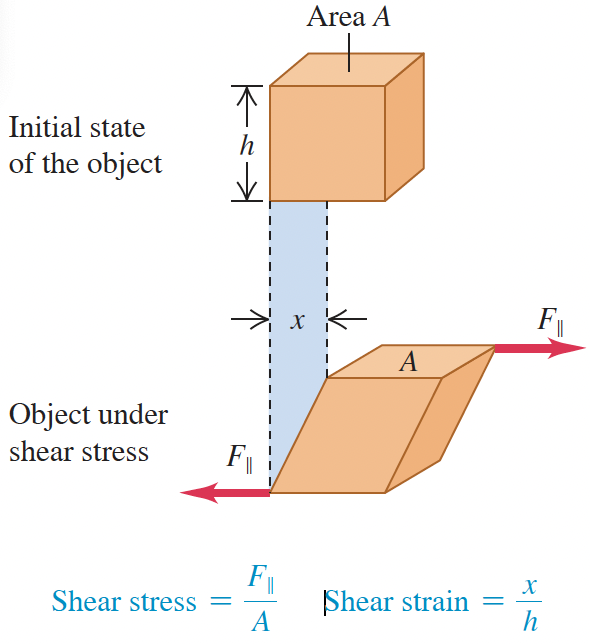
\includegraphics[width=0.2\linewidth]{../figures/F2.png}
  \label{fig:F2}
\end{figure}

Forskydningsmodulet $S$ kan findes som
\[ 
S = \frac{\sigma_{\text{forskydning}}}{\epsilon_{\text{forskydning}}} = \frac{F_{\parallel} / A}{x / h} = \frac{F_{\parallel}}{A} \frac{h}{x}
.\]
Hvor $F_{\parallel}$ er kraften der påføres parallelt med ovjektets overflade, $A$ er arealet som kraften arbejder over, $x$ er deformationen og $h$ er den tværgående afstand (se evt. \textbf{\autoref{fig:F2}} fra bogens side 350).


\subsection{Perturbationsteoretisk ligevægt}
Fra perturbationsteori har vi at et system i ligevægt er stabilt (en lille ændring i systemet ødelægger ikke ligevægten) såfremt
\[ 
\frac{\mathrm{d}U^2}{\mathrm{d}^2x} > 0
,\]
Hvor $U$ er potentiel energi og $x$ er position. Dette resultat gælder eftersom enhver lille forskydning af massen dx i dette tilfælde medfører en restaurerende kraft og vice versa.
